\section{Aspen Plus Configuration}

\begin{enumerate}
	\item The initial steps for opening a simulation and entering metadata for an Aspen Plus simulation are similar to ACM. Refer to the SimSinter ACM tutorial \ref{sec.tut.simsinter.acm}. In this tutorial, a flash model ``Flash\_Example.bkp'' installed in the ``C:\textbackslash SimSinterFiles\textbackslash Aspen\_Plus\_Install\_Test'' is used as an example. Open the Aspen Plus file and enter the metadata as shown in Figure \ref{fig.sinter.ap.metadata}.
  \begin{figure}[H]
	\begin{center}
		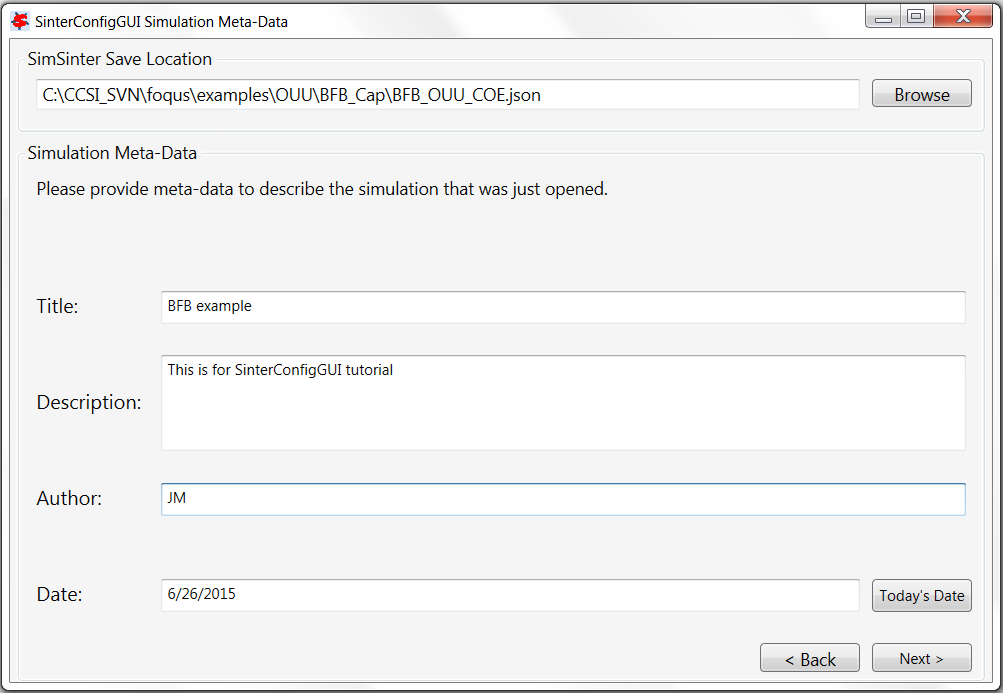
\includegraphics[scale=0.55]{Chapt_sinter/figs/ap/04_MetaDataFilled}
		\caption{SinterConfigGUI Simulation Meta-Data with Data Completed}
		\label{fig.sinter.ap.metadata}
	\end{center}
  \end{figure}
  
\item The \textbf{\underline{SinterConfigGUI Variable Configuration Page}} displays as illustrated in Figure \ref{fig.sinter.ap.variableempty}. Aspen Plus has no settings, so there are no setting variables in the input
  section. Unlike ACM, AspenPlus displays the \textbf{\underline{Variable Tree}} on the
  left side, so the user can explore the tree as is done in Aspen Plus
  Tools $\rightarrow$ Variable Explorer.  Unfortunately, searching is not possible.
  \begin{figure}[H]
	\begin{center}
		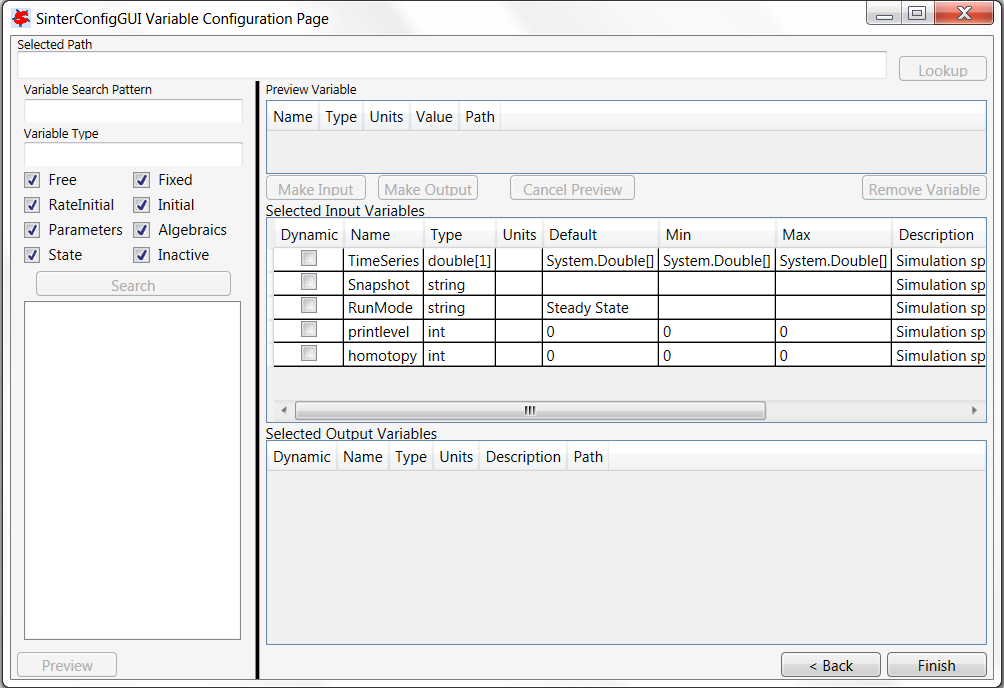
\includegraphics[scale=0.55]{Chapt_sinter/figs/ap/05_VariablesEmpty}
		\caption{SinterConfigGUI Variable Configuration Page Empty Variables}
		\label{fig.sinter.ap.variableempty}
	\end{center}
  \end{figure}

\item \textbf{\underline{Variable Tree}} nodes can be expanded for searching (Figure \ref{fig.sinter.ap.expandtree}).
  \begin{figure}[H]
	\begin{center}
		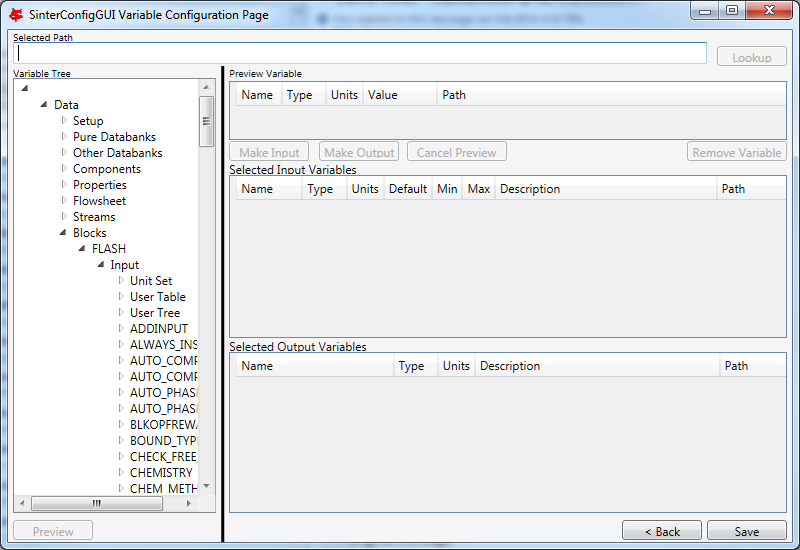
\includegraphics[scale=0.55]{Chapt_sinter/figs/ap/06_VariablesExpanded}
		\caption{SinterConfigGUI Variable Configuration Page Expanded Aspen Plus Variable Tree}
		\label{fig.sinter.ap.expandtree}
	\end{center}
  \end{figure}
  
\item The user can type the node address directly into the \textbf{\underline{Selected Path}} field (this is useful for copy/paste from Aspen Plus' Variable Explorer) (Figure \ref{fig.sinter.ap.selectvar}). Click \textbf{\underline{Lookup}} or \textbf{\underline{Preview}} (which automatically causes the tree to expand and selects selected variables in the \textbf{\underline{Variable Tree}}).
  \begin{figure}[H]
	\begin{center}
		\includegraphics[scale=0.55]{Chapt_sinter/figs/ap/07_VariablesSelected}
		\caption{SinterConfigGUI Variable Configuration Page Aspen Plus Variable Selected}
		\label{fig.sinter.ap.selectvar}
	\end{center}
  \end{figure}
%\clearpage
\item To make the temperature of the Flash chamber an \textbf{\underline{Input Variable}}, click \textbf{\underline{Make Input}}. Additionally, the user can \textbf{\underline{Name}} the variable, fix the \textbf{\underline{Description}}, and enter the \textbf{\underline{Min/Max}} fields by clicking on the appropriate text and entering it.
  \begin{figure}[H]
	\begin{center}
		\includegraphics[scale=0.55]{Chapt_sinter/figs/ap/08_VariablesInput}
		\caption{SinterConfigGUI Variable Configuration Page Input Variable}
		\label{fig.sinter.ap.inputvar}
	\end{center}
  \end{figure}
%\clearpage
\item Select an \textbf{\underline{Output Variable}}, \textbf{\underline{Preview}} it, and click \textbf{\underline{Make Output}}. Next, update the fields as with the \textbf{\underline{Input Variable}} to give a better \textbf{\underline{Name}} and \textbf{\underline{Description}}.
  \begin{figure}[H]
	\begin{center}
		\includegraphics[scale=0.55]{Chapt_sinter/figs/ap/09_VariablesOutput}
		\caption{SinterConfigGUI Variable Configuration Page Output Variable}
		\label{fig.sinter.ap.outputvar}
	\end{center}
  \end{figure}
\item The task is complete. Save it by clicking \textbf{\underline{Save}} or CTRL+S. The file is saved to the location specified in the
  SinterConfigGUI Simulation Meta-Data page. If the user wishes to save a copy under a different name,
  navigate back to the SinterConfigGUI Simulation Meta-Data page and change the name. 
\end{enumerate}
